\chapter{Handover}

It is important that all Engineers are aware of the original scope of works. The original scope of works can be found here.

Responsibility for raising the issue of V.O.'s is as follows:

\begin{figure}
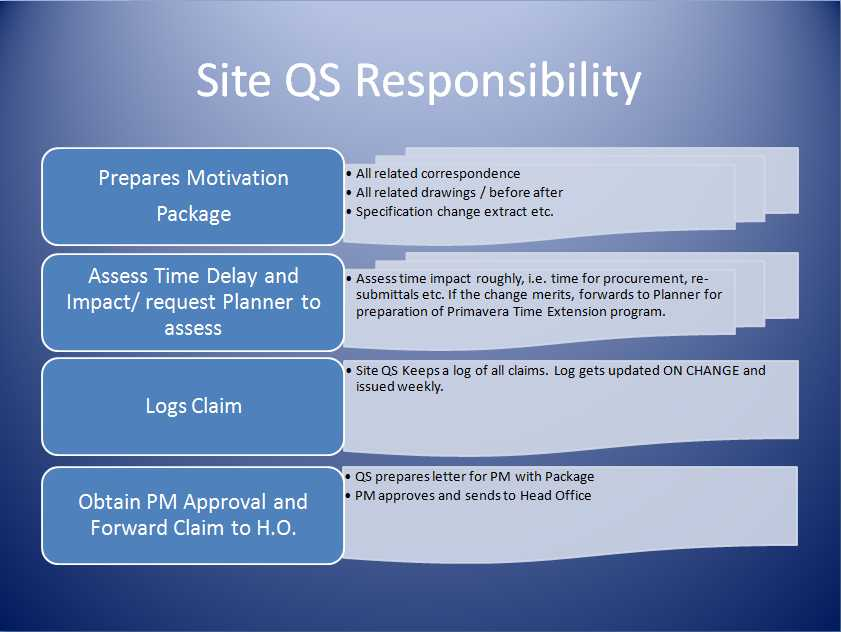
\includegraphics[width=1.3\textwidth]{./graphics/Site-QS-responsibilities}
\end{figure}

\section*{Hand Over Documentation}

The aim of collating all documentation at the end of a Project in order to verify that all parties have inspected and accepted the Installation. These documentation will have to be enclosed in the Operations and Maintenance Manuals.

\section*{As-Build Drawings}

This is the most basic requirements and in an ideal Site they will be produced as an on-going activity, while the Site is operating. Remember that every change on the AS-BUILDS points to lack of good engineering at the beginning of the Project and to an extent lack of planning. Minor changes are understandable to incorporate Site instructions but any large scale operations to update drawings is as a sad story.

\section*{Proof that the Works have been Physically Inspected}

A list of all WIR's properly collated should be summarized.
Contractor's confirmation that the works have been completed.

\section*{Proof of commissioning}


\section*{The Final Touch}

Depending on the specification, the Designers might have even elected to
specify the font and the font-sizes for the manual. The OM manuals will
impact on our brand long after we have left the project. It is important that
they look professional and that they are bound correctly. Drawings and CDs
should be copied properly.










